\documentclass[a4paper]{article}
\usepackage[utf8]{inputenc}
\usepackage{graphicx}
\usepackage{amsmath}
\usepackage[bottom=2.0cm,top=2.0cm,left=2.0cm,right=2.0cm]{geometry}
\usepackage[english]{babel}
\usepackage{indentfirst}
\usepackage{hyperref}  
\hypersetup{colorlinks,citecolor=black,filecolor=black,linkcolor=black,urlcolor=black}
\usepackage[nottoc]{tocbibind}
\usepackage{lipsum}
\usepackage{blindtext}
\usepackage{pdfpages}
\usepackage{epsfig} %% for loading postscript figures
\usepackage{listings}
\usepackage{hyperref}
\usepackage{amssymb}
\usepackage{setspace}
\usepackage{fancyhdr}
\usepackage{cite}
\usepackage{caption}
\usepackage{subcaption}
\usepackage{float}


\pagestyle{fancy}
\fancyhf{}
\renewcommand{\headrulewidth}{0pt}

\rfoot{\thepage \hspace{1pt}}

\doublespace
\begin{document}
\title{Engineering Report}


\begin{titlepage}
	\begin{center}
		\begin{figure}[htb!]
			\begin{flushleft}
				
\includegraphics[width=3.9cm]{images/fau_logo.jpeg}
			\end{flushleft}
		\end{figure}
        \vspace{-2.5cm}
        \hspace{2.1cm}\Large{\textbf{Florida Atlantic University}}\\
        \hspace{2.1cm}\Large{College of Engineering}\\
        
        \vspace{200pt}
        
        \LARGE{\textbf{Project 1}}\\ 
        \Large{Application of the Direct Integration Method or of Discontinuity (Singularity) Functions to Statically Determinate Uniform or Stepped Beam Design}\\ 
        
        \vspace{100pt}
        
        \hfill Serial Number: 02 \\
        
        \vspace{30pt} 
        \hfill Name: Pedro Almeida\\
        \hfill Professor Name: Dr. Isaac Elishakoff\\
        \hfill TA Name: Abhishek Ratanpara\\
        \hfill Student Email: palmeida2016@fau.edu\\
        \hfill Telephone Number: +1 (561) 480-5483\\
        
        
        \vspace{\fill}
        \LARGE \bf{\today}
          
	\end{center}
\end{titlepage}


\includepdf[pages=-]{assignment/project1_probs.pdf}
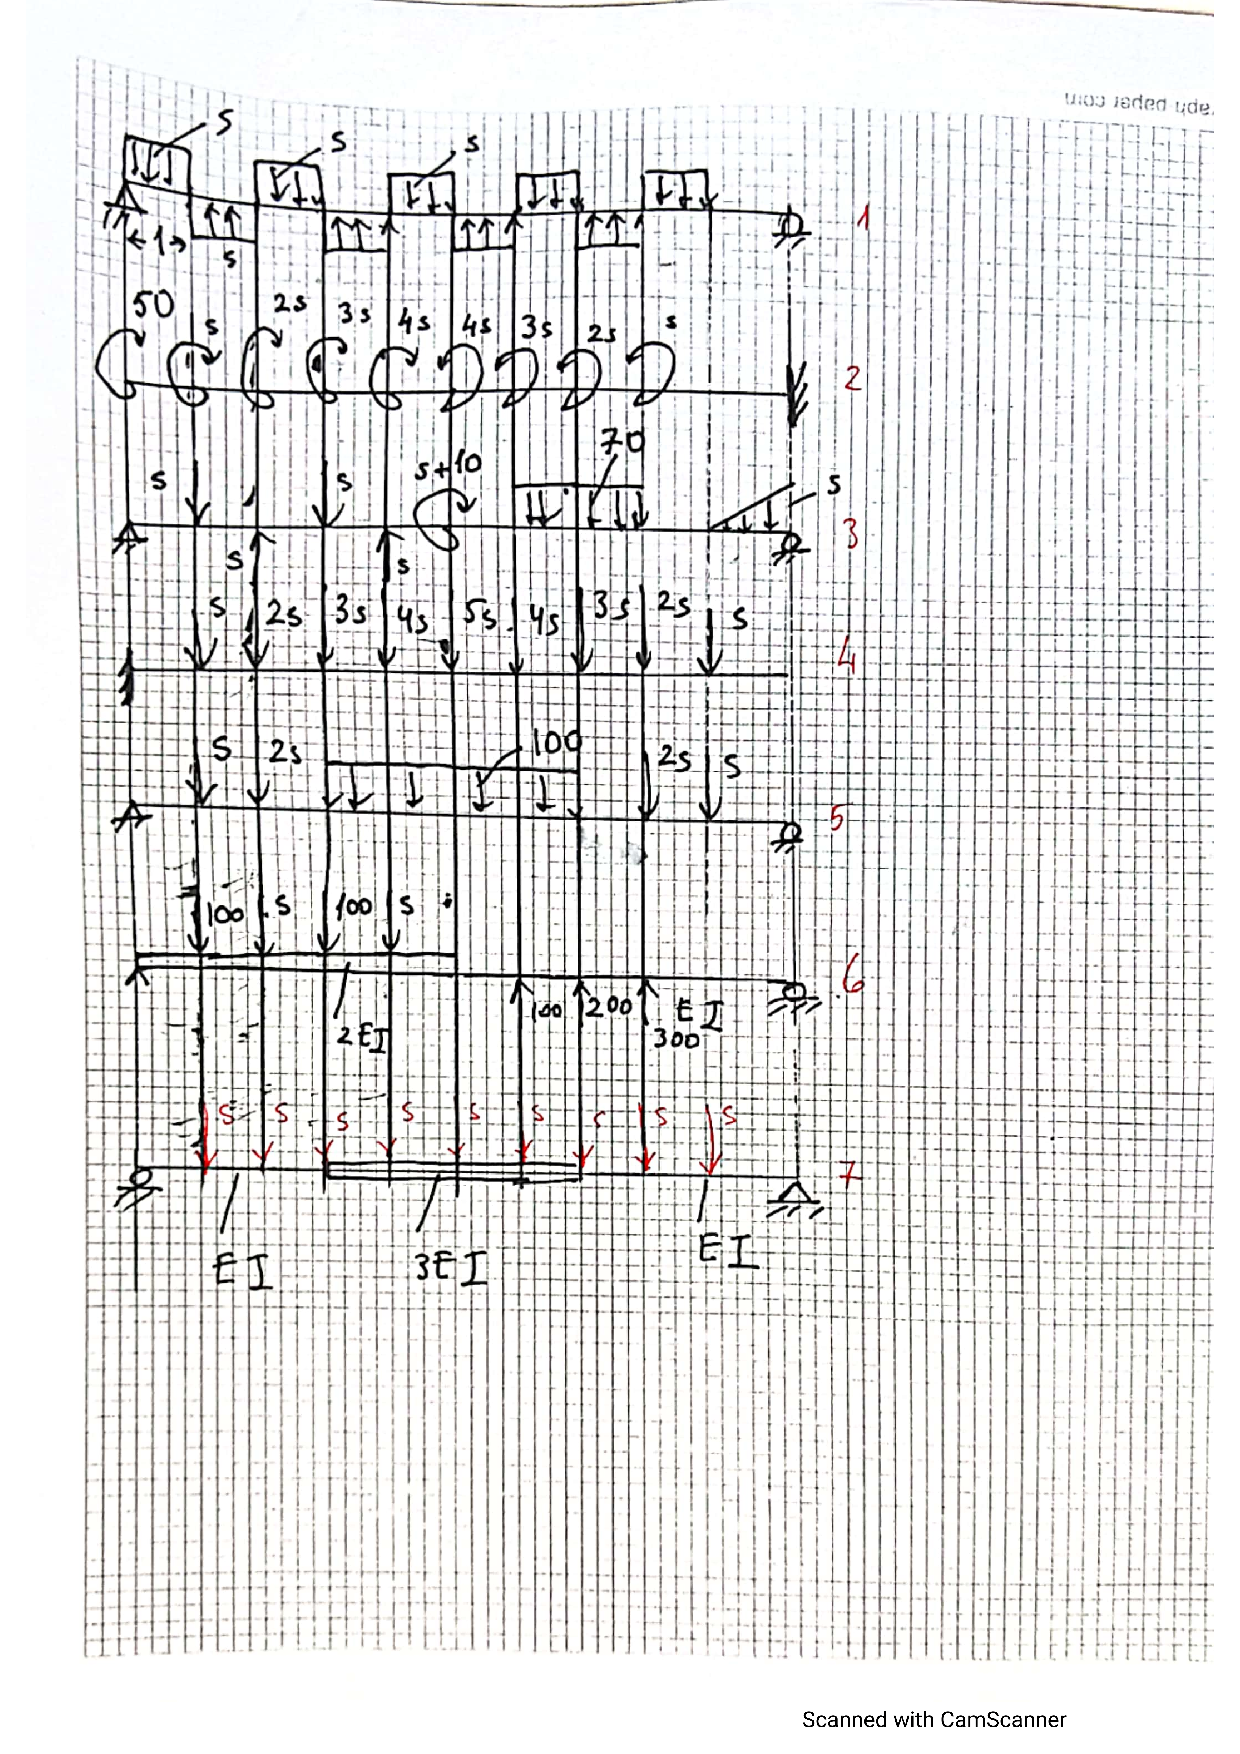
\includepdf[pages=-]{assignment/project1_dwg.pdf}

\large
\textit{The report will apply the Direct Integration Method of Singularity Functions to statically determine uniform or stepped beam designs to determine the load's effect on the beam's deflection. The resulting functions following the integration will be plotted using MATLAB software to produce simplified renderings of the beam's shape post loading.}

\tableofcontents

\section{Introduction} \label{Introduction}
One of the most important processes in designing beams is the structural analysis of the part under realistic loading conditions. A proper, realistic, theoretical model allows the engineer or designer to understand the expected stresses and deflections of a beam under expected loading conditions, thus removing the need to conduct experiments for each attempted revision. To properly construct the theoretical models, engineers often rely on extensive sets of equations.

The standard method to solve for beam deflection for beams with continuous cross sectional areas relies on partitions; the designer splits the beam into multiple subsections where loads are applied. The resulting cross sections are then each modeled separately. The singularity equations for beam deflection, by contrast, allow for the reduction of the multiple deflection equations into a single continuous equation. The method will be discussed thoroughly in the \nameref{Background Theory} section.

The report will comprise of the \nameref{Background Theory} section discussing the required equations and methods to solve the problems, the \nameref{Problems} section discussing each of the problems presented in the project, \nameref{Results} where problem solutions are discussed, and the \nameref{Conclusions} section to summarize findings and discuss improvements.

\section{Background Theory} \label{Background Theory}
To find the deflection equation for a statically determinate beam under loading, there are two principal ways to approach the problem, both of which lead to the same result \cite{book}. The first method, shown in Eq. \ref{form1}, uses the loading function $w(x)$ to reach the deflection. The form is especially useful for beams under non-linear loading functions. However, due to the required quadruple integration to reach $v(x)$, engineers commonly use a second form.

\begin{equation}
    EI \frac{\delta^4 v}{\delta x^4} = w(x)
\label{form1}
\end{equation}

The second form of the deflection equation can be given by Eq. \ref{form3}. The function utilizes the moment function $W(x)$ and a double integration to model the deflection, generating 2 constants of integration rather than 4. As such, if possible, the second form is preferred. With the form of integration determined, the engineering must then determine the moment function applied onto the beam as a function of the loads, which begins by statically solving the problem.

\begin{equation}
    EI \frac{\delta^2 v}{\delta x^2} = M(x)
\label{form3}
\end{equation}

The first step to find the static forces acting on a beam includes the decomposition of the applied and reaction forces onto a Free Body Diagram (FBD). To define the FBD, the report must first determine the type of supports acting on the beam. For a simply supported beam, the pin support creates a reaction $x$ and $y$ directions, while the roller support only creates a reaction in the $y$ direction. For a wall support, the beam must have a reaction in the $x$ and $y$ directions in addition to a moment reaction. Fig. \ref{FBD_example} shows an example of a FBD decomposition.

\begin{figure}[h]
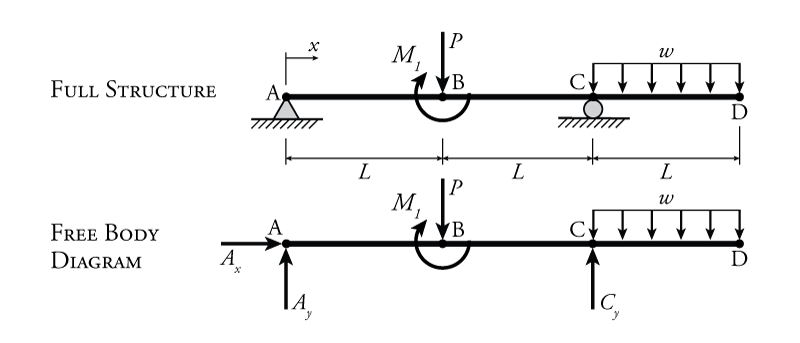
\includegraphics[width=\textwidth]{FBD/FBD_example.jpeg}
\caption{Example Free Body Diagram}
\label{FBD_example}
\end{figure}

With the FBD drawn, the report uses the set of equations shown in Eq. \ref{static_equations} to solve for the reaction forces. In most scenarios, the horizontal force $F_x$, and therefore the horizontal reaction, will be equal to zero, leaving 2 main equations to be used to solve for the vertical reactions at each of the supports. 

\begin{equation}
    \begin{split}
    &\uparrow \sum F_y = 0 \\
    &\rightarrow \sum F_x = 0 \\
    &\circlearrowleft \sum M_A = 0
    \end{split}
\label{static_equations}
\end{equation}

Once the support reactions have been found, the engineer proceeds by selecting Eq. \ref{form1} or Eq. \ref{form3} to apply. For the purposes of the example, Eq. \ref{form3} will be used. For that form, the report sets an $x$-$y$ coordinate system on the left side of the beam such that the $x$ axis extends along the beam and the $y$ axis extends perpendicular to the length of the beam. With the coordinate system established, the report constructs the Moment equation based on Eq. \ref{moment_equation} where the moment $M$ can be found as the product of the force $F$ and the radius of the arm $r$ given as the distance between the force to the axis of rotation.

\begin{equation}
    M = F * r
\label{moment_equation}
\end{equation}

For the given example, the moment equation is as shown in Eq. \ref{moment_equation_example}. In the equation, any term found containing $<x-x_0>^n$ conveys the force represented only acts starting from point $x_0$; that is, if the beam were to be segmented prior to $x_0$ such that $x<x_0$, the moment generated would be equal to zero. As such, $<x-x_0>^n$ evaluates to $(x-x_0)^n$ if $x>=x_0$ or $0$ if $x<x_0$.

\begin{equation}
    M(x) = -P\left<x-L\right>^1 - M_I\left<x-L\right>^0 + C_y\left<x-2L\right>^1 - \frac{w}{2}\left<x-2L\right>^2
\label{moment_equation_example}
\end{equation}

With the moment equation found, the report will integrate it twice as given per Eq. \ref{form3} to find $v(x)$, which can be shown in Eq. \ref{moment_equation_example_int}.

\begin{equation}
    \begin{split}
    & EI \frac{\delta^2 v}{\delta x^2} = -P\left<x-L\right>^1 - M_I\left<x-L\right>^0 + C_y\left<x-2L\right>^1 - \frac{w}{2}\left<x-2L\right>^2 \\
    & EI \frac{\delta v}{\delta x} = \frac{-P}{2}\left<x-L\right>^2 - M_I\left<x-L\right>^1 + \frac{C_y}{2}\left<x-2L\right>^2 -  \frac{w}{6}\left<x-2L\right>^3 + C_1\\
    & EI v(x) = \frac{-P}{6}\left<x-L\right>^3 - \frac{M_I}{2}\left<x-L\right>^2 + \frac{C_y}{6}\left<x-2L\right>^3 - \frac{w}{24}\left<x-2L\right>^4 + C_1 x + C_2
    \end{split}
\label{moment_equation_example_int}
\end{equation}

The last step in finding the displacement equation is to apply the boundary conditions to find the coefficients of integration $C_1$ and $C_2$, which use the properties of the supports. As given in Fig. \ref{FBD_example}, there are two supports that provide vertical reactions to the beam's displacement. In other words, at the point of contact with each of the supports, the vertical displacement must be equal to zero. As such, we can use the conditions shown in Eqs. \ref{moment_equation_example_coef1} and \ref{moment_equation_example_coef2} to solve for $C_1$ and $C_2$.

\begin{equation}
    \begin{split}
    	& v(x=0) = 0  \\
 	& \Rightarrow \frac{-P}{6}\left<(0)-L\right>^3 - \frac{M_I}{2}\left<(0)-L\right>^2 + \frac{C_y}{6}\left<(0)-2L\right>^3 - \frac{w}{24}\left<(0)-2L\right>^4 + C_1 (0) + C_2 \\
	& \Rightarrow C_2 = 0 \\
    \end{split}
\label{moment_equation_example_coef1}
\end{equation}

\begin{equation}
    \begin{split}
	& v(x=2L) = 0  \\
 	& \Rightarrow \frac{-P}{6}\left<(2L)-L\right>^3 - \frac{M_I}{2}\left<(2L)-L\right>^2 + \frac{C_y}{6}\left<(2L)-2L\right>^3 - \frac{w}{24}\left<(2L)-2L\right>^4 + C_1 (2L) + C_2 \\
	& \Rightarrow C_1 = \frac{\frac{PL^3}{6} + \frac{M_I L^2}{2}}{2L} = \frac{PL^2}{12} + \frac{M_I L}{4} \\
    \end{split}
\label{moment_equation_example_coef2}
\end{equation}

Therefore, the final equation for the deflection of the beam can be found as shown in Eq. \ref{moment_equation_example_final} where the unknown coefficients have been solved for.

\begin{equation}
EI v(x) = \frac{-P}{6}\left<x-L\right>^3 - \frac{M_I}{2}\left<x-L\right>^2 + \frac{C_y}{6}\left<x-2L\right>^3 - \frac{w}{24}\left<x-2L\right>^4 + \left( \frac{PL^2}{12} + \frac{M_I L}{4} \right) x
\label{moment_equation_example_final}
\end{equation}




\section{Problem Definition} \label{Problems}
\subsection{Problem 1}

As given by the project assignment, the first project constitutes of a simply supported beam subject to a series of area loads as shown in Fig. \ref{prob1:prob}. By substituting the equivalent reaction forces, the report generates the FBD shown in Fig. \ref{prob1:FBD}.


With the Free-Body Diagram completed, the report employs the static equations to find the reaction forces at each of the supports as shown in Eq. \ref{problem1_reaction_equation}.

\begin{equation}
\begin{split}
	&\uparrow \sum F_y = R_a - 2(1) + 2(1) - 2(1) + 2(1) - 2(1) + 2(1) - 2(1) + 2(1) - 2(1) + R_b = 0 \\
 	&\rightarrow \sum F_x = 0 \\
 	&\circlearrowleft \sum M_A = -2(1)\left(\frac{1}{2}\right) + 2(1)\left(\frac{3}{2}\right) - 2(1)\left(\frac{5}{2}\right) + 2(1)\left(\frac{7}{2}\right) - 2(1)\left(\frac{9}{2}\right) + 2(1)\left(\frac{11}{2}\right) \\ 
	& - 2(1)\left(\frac{13}{2}\right) + 2(1)\left(\frac{15}{2}\right) - 2(1)\left(\frac{17}{2}\right) + R_b(10) = 0 \\
\end{split}
\label{problem1_reaction_equation}
\end{equation}

Given the problem is statically determinate, the static equations are sufficient to find the reaction forces for the supports, which are shown in Eq. \ref{problem1_reaction_solution}. Since there are no horizontal forces applied, the only non-zero reactionary forces are those in the vertical direction, which will be named $R_a$ and $R_b$ henceforth.

\begin{equation}
\begin{split}
	& R_b = \frac{9}{10} \\
	& R_a = \frac{11}{10} \\
\end{split}
\label{problem1_reaction_solution}
\end{equation}

With the reactions determined, the moment and deflection equations can be constructed as shown in Eq. \ref{problem1_equations}.

\begin{equation}
    \begin{split}
& EI \frac{\delta^2 v}{\delta x^2} = \frac{11}{10}\left<x-0\right>^1 - \left<x-0\right>^2 +  2\left<x-1\right>^2 - 2\left<x-2\right>^2 +  2\left<x-3\right>^2 - 2\left<x-4\right>^2  \\
& +  2\left<x-5\right>^2 - 2\left<x-6\right>^2  +  2\left<x-7\right>^2 - 2\left<x-8\right>^2 + \left <x-9\right>^2 \\
& \\
& EI \frac{\delta v}{\delta x} =  \frac{11}{20}\left<x-0\right>^2 - \frac{1}{3}\left<x-0\right>^3 +  \frac{2}{3}\left<x-1\right>^3 - \frac{2}{3}\left<x-2\right>^3 +  \frac{2}{3}\left<x-3\right>^3 - \frac{2}{3}\left<x-4\right>^3 \\
&  +  \frac{2}{3}\left<x-5\right>^3 - \frac{2}{3}\left<x-6\right>^3  +  \frac{2}{3}\left<x-7\right>^3 - \frac{2}{3}\left<x-8\right>^3 +  \frac{1}{3}\left<x-9\right>^3 + C_1\\
& \\
& EI v(x) = \frac{11}{60}\left<x-0\right>^3 - \frac{1}{12}\left<x-0\right>^4 +  \frac{1}{6}\left<x-1\right>^4 - \frac{1}{6}\left<x-2\right>^4 + \frac{1}{6}\left<x-3\right>^4 - \frac{1}{6}\left<x-4\right>^4  \\      
& +  \frac{1}{6}\left<x-5\right>^4 - \frac{1}{6}\left<x-6\right>^4  +  \frac{1}{6}\left<x-7\right>^4 - \frac{1}{6}\left<x-8\right>^4 +  \frac{1}{12}\left<x-9\right>^4 + C_1x + C_2 \\
    \end{split}
\label{problem1_equations}
\end{equation}

Following the integration of the singularity moment equation, the report solves for the two constants of integration through the use of boundary conditions. As given in the problem description, the two vertical supports at A and B guarantee the deflection at these points is equal to zero, as shown in Eq. \ref{problem1_constants_of_integration}

\begin{equation}
\begin{split}
	& v(0) = 0 \\
	& v(10) = 0 \\
\end{split}
\label{problem1_constants_of_integration}
\end{equation}

Using the boundary conditions shown above, the report finds the constants of integration to the values shown in Eq. \ref{problem1_constants_of_integration_solution}.

\begin{equation}
\begin{split}
	& C_2 = 0 \\
	& C_1 = \frac{209}{240} \\
\end{split}
\label{problem1_constants_of_integration_solution}
\end{equation}

After plugging in the boundary conditions, the report finds the deflection equation shown in Eq. \ref{problem1_final_equation}.

\begin{equation}
\begin{split}
  & EI v(x) = \frac{11}{60}\left<x-0\right>^3 - \frac{1}{12}\left<x-0\right>^4 +  \frac{1}{6}\left<x-1\right>^4 - \frac{1}{6}\left<x-2\right>^4 + \frac{1}{6}\left<x-3\right>^4 - \frac{1}{6}\left<x-4\right>^4 \\  	  
&   +  \frac{1}{6}\left<x-5\right>^4 - \frac{1}{6}\left<x-6\right>^4  +  \frac{1}{6}\left<x-7\right>^4 - \frac{1}{6}\left<x-8\right>^4 +  \frac{1}{12}\left<x-9\right>^4 + \frac{209}{240}x\\
\end{split}
\label{problem1_final_equation}
\end{equation}

\subsection{Problem 2}

As given by the project assignment, the first project constitutes of a simply supported beam subject to a series of area loads. By substituting the equivalent reaction forces, the report generates the FBD shown in Fig. \ref{prob2:FBD}.

With the Free-Body Diagram completed, the report employs the static equations to find the reaction forces at each of the supports as shown in Eq. \ref{problem2_reaction_equation}.

\begin{equation}
\begin{split}
	&\uparrow \sum F_y = R_{ay} = 0 \\
 	&\rightarrow \sum F_x = R_{ax} = 0 \\
 	&\circlearrowleft \sum M_A = -50 - 2 - 4 - 6 - 8 + 8 + 6 + 4 + 2 + M_a = 0
\end{split}
\label{problem2_reaction_equation}
\end{equation}

Given the problem is statically determinate, the static equations are sufficient to find the reaction forces for the supports, which are shown in Eq. \ref{problem2_reaction_solution}. Since there are no horizontal forces applied, the only non-zero reaction is the reactionary moment, which will be named $M_a$ henceforth.

\begin{equation}
\begin{split}
	& M_a = 50 \\
	& R_{ax} = 0 \\
	& R_{ay} = 0 \\
\end{split}
\label{problem2_reaction_solution}
\end{equation}

With the reactions determined, the moment and deflection equations can be constructed as shown in Eq. \ref{problem2_equations}.

\begin{equation}
    \begin{split}
& EI \frac{\delta^2 v}{\delta x^2} = 50\left<x-0\right>^0 + 2\left<x-1\right>^0 + 4\left<x-2\right>^0 + 6\left<x-3\right>^0 + 8\left<x-4\right>^0   -  8\left<x-5\right>^0 \\
& - 6\left<x-6\right>^0 -  4\left<x-7\right>^0 - 2\left<x-8\right>^0 \\
& \\
& EI \frac{\delta v}{\delta x} = 50\left<x-0\right>^1 + 2\left<x-1\right>^1 + 4\left<x-2\right>^1 +  6\left<x-3\right>^1 + 8\left<x-4\right>^1   -  8\left<x-5\right>^1 \\
& - 6\left<x-6\right>^1 -  4\left<x-7\right>^1 - 2\left<x-8\right>^1 + C_1 \\
& \\
& EI v(x) = 25\left<x-0\right>^2 + \left<x-1\right>^2 + 2\left<x-2\right>^2 +  3\left<x-3\right>^2 + 4\left<x-4\right>^2   -  4\left<x-5\right>^2 \\
& - 3\left<x-6\right>^2  -  2\left<x-7\right>^2 - \left<x-8\right>^2 + C_1 x + C_2 \\
    \end{split}
\label{problem2_equations}
\end{equation}

Following the integration of the singularity moment equation, the report solves for the two constants of integration through the use of boundary conditions. As given in the problem description, the fixed at A guarantees the deflection and slope at A is equal to zero, as shown in Eq. \ref{problem2_constants_of_integration}.

\begin{equation}
\begin{split}
	& v(10) = 0 \\
	& \frac{\delta v(10)}{\delta x} = 0 \\
\end{split}
\label{problem2_constants_of_integration}
\end{equation}

Using the boundary conditions shown above, the report finds the constants of integration to the values shown in Eq. \ref{problem2_constants_of_integration_solution}.

\begin{equation}
\begin{split}
	& C_2 = 2770 \\
	& C_1 = -560 \\
\end{split}
\label{problem2_constants_of_integration_solution}
\end{equation}

After plugging in the boundary conditions, the report finds the deflection equation shown in Eq. \ref{problem2_final_equation}.

\begin{equation}
\begin{split}
  & EI v(x) = 25\left<x-0\right>^2 + \left<x-1\right>^2 + 2\left<x-2\right>^2 + 3\left<x-3\right>^2 + 4\left<x-4\right>^2  -  4\left<x-5\right>^2 \\
& - 3\left<x-6\right>^2  -  2\left<x-7\right>^2 - \left<x-8\right>^2 - 560 x + 2770 \\
\end{split}
\label{problem2_final_equation}
\end{equation}



\subsection{Problem 3}

As given by the project assignment, the first project constitutes of a simply supported beam subject to a series of area loads. By substituting the equivalent reaction forces, the report generates the FBD shown in Fig. \ref{prob3:FBD}.

With the Free-Body Diagram completed, the report employs the static equations to find the reaction forces at each of the supports as shown in Eq. \ref{problem3_reaction_equation}.

\begin{equation}
\begin{split}
	&\uparrow \sum F_y = R_a - 2 + 2 - 2 + 2 - 70(2) - 2(1)\left(\frac{1}{2}\right) + R_b = 0 \\
 	&\rightarrow \sum F_x = R_{ax} = 0 \\
 	&\circlearrowleft \sum M_A = -2(1) + 2(2) - 2(3) + 2(4) - 12 - 70(2)(7) - 2(1)\left(\frac{29}{6}\right) + R_{by}(10) = 0 \\
\end{split}
\label{problem3_reaction_equation}
\end{equation}

Given the problem is statically determinate, the static equations are sufficient to find the reaction forces for the supports, which are shown in Eq. \ref{problem3_reaction_solution}. Since there are no horizontal forces applied, the only non-zero reactionary forces are those in the vertical direction, which will be named $R_a$ and $R_b$ henceforth.

\begin{equation}
\begin{split}
	& R_b = \frac{2993}{30} \\
	& R_a = \frac{1237}{30} \\
\end{split}
\label{problem3_reaction_solution}
\end{equation}

With the reactions determined, the moment and deflection equations can be constructed as shown in Eq. \ref{problem3_equations}.

\begin{equation}
    \begin{split}
& EI \frac{\delta^2 v}{\delta x^2} = \frac{1237}{30}\left<x-0\right>^1 - 2\left<x-1\right>^1 +  2\left<x-2\right>^1 - 2\left<x-3\right>^1 +  2\left<x-4\right>^1 \\
& + 12\left<x-5\right>^0 -  35\left<x-6\right>^2 + 35\left<x-8\right>^2  - \frac{1}{3}\left<x-9\right>^3 \\
& \\
& EI \frac{\delta v}{\delta x} = \frac{1237}{60}\left<x-0\right>^2 - \left<x-1\right>^2 +  \left<x-2\right>^2 - \left<x-3\right>^2 +  \left<x-4\right>^2 + 12\left<x-5\right>^1\\
& -  \frac{35}{3}\left<x-6\right>^3 + \frac{35}{3}\left<x-8\right>^3  - \frac{1}{12}\left<x-9\right>^4 + C_1 \\
& \\
& EI v(x) =\frac{1237}{180}\left<x-0\right>^3 - \frac{1}{3}\left<x-1\right>^3 +  \frac{1}{3}\left<x-2\right>^3 - \frac{1}{3}\left<x-3\right>^3 +  \frac{1}{3}\left<x-4\right>^3\\
& + 6\left<x-5\right>^2 -  \frac{35}{12}\left<x-6\right>^4 + \frac{35}{12}\left<x-8\right>^4  - \frac{1}{60}\left<x-9\right>^5 + C_1x + C_2 \\ \\
    \end{split}
\label{problem3_equations}
\end{equation}

Following the integration of the singularity moment equation, the report solves for the two constants of integration through the use of boundary conditions. As given in the problem description, the two vertical supports at A and B guarantee the deflection at these points is equal to zero, as shown in Eq. \ref{problem3_constants_of_integration}.

\begin{equation}
\begin{split}
	& v(0) = 0 \\
	& v(10) = 0 \\
\end{split}
\label{problem3_constants_of_integration}
\end{equation}

Using the boundary conditions shown above, the report finds the constants of integration to the values shown in Eq. \ref{problem3_constants_of_integration_solution}.

\begin{equation}
\begin{split}
	& C_2 = 0 \\
	& C_1 = \frac{-1117357}{1800} \\
\end{split}
\label{problem3_constants_of_integration_solution}
\end{equation}

After plugging in the boundary conditions, the report finds the deflection equation shown in Eq. \ref{problem3_final_equation}.

\begin{equation}
\begin{split}
  & EI v(x) = \frac{1237}{180}\left<x-0\right>^3 - \frac{1}{3}\left<x-1\right>^3 +  \frac{1}{3}\left<x-2\right>^3 - \frac{1}{3}\left<x-3\right>^3 +  \frac{1}{3}\left<x-4\right>^3\\
& + 6\left<x-5\right>^2 -  \frac{35}{12}\left<x-6\right>^4 + \frac{35}{12}\left<x-8\right>^4  - \frac{1}{60}\left<x-9\right>^5 + \frac{-1117357}{1800}x\\
\end{split}
\label{problem3_final_equation}
\end{equation}





\subsection{Problem 4}

As given by the project assignment, the first project constitutes of a simply supported beam subject to a series of area loads. By substituting the equivalent reaction forces, the report generates the FBD shown in Fig. \ref{prob4:FBD}.

With the Free-Body Diagram completed, the report employs the static equations to find the reaction forces at each of the supports as shown in Eq. \ref{problem4_reaction_equation}.

\begin{equation}
\begin{split}
	&\uparrow \sum F_y = R_{ay} -2 -4 -6 -8 -10 -8 -6 -4 -2 = 0 \\
 	&\rightarrow \sum F_x = R_{ax} = 0 \\
 	&\circlearrowleft \sum M_A = M_a -2(1) -4(2) -6(3) -8(4) -10(5) -8(6) -6(7)- 4(8) -2(9) = 0
\end{split}
\label{problem4_reaction_equation}
\end{equation}

Given the problem is statically determinate, the static equations are sufficient to find the reaction forces for the supports, which are shown in Eq. \ref{problem4_reaction_solution}. Since there are no horizontal forces applied, the only non-zero reactions are the reactionary moment and vertical reaction, which will be named $M_a$ and $R_a$ henceforth.

\begin{equation}
\begin{split}
	& M_a = -250 \\
	& R_{ax} = 0 \\
	& R_{ay} = 50 \\
\end{split}
\label{problem4_reaction_solution}
\end{equation}

With the reactions determined, the moment and deflection equations can be constructed as shown in Eq. \ref{problem4_equations}.

\begin{equation}
    \begin{split}
& EI \frac{\delta^2 v}{\delta x^2} = 50\left<x-0\right>^1 - 250\left<x-0\right>^0 - 2\left<x-1\right>^1 - 4\left<x-2\right>^1 - 6\left<x-3\right>^1 - 8\left<x-4\right>^1 \\
& - 10\left<x-5\right>^1 -  8\left<x-6\right>^1 - 6\left<x-7\right>^1 -  4\left<x-8\right>^1 - 2\left<x-9\right>^1 \\
& \\
& EI \frac{\delta v}{\delta x} = 25\left<x-0\right>^2 - 250\left<x-0\right>^1 - \left<x-1\right>^2 - 2\left<x-2\right>^2 - 3\left<x-3\right>^2 - 4\left<x-4\right>^2\\
& - 5\left<x-5\right>^2 -  4\left<x-6\right>^2 - 3\left<x-7\right>^2 -  2\left<x-8\right>^2 - \left<x-9\right>^2 + C_1 \\
& \\
& EI v(x) = \frac{25}{6}\left<x-0\right>^3 - 125\left<x-0\right>^2 - \frac{1}{3}\left<x-1\right>^3 - \frac{2}{3}\left<x-2\right>^3 - \left<x-3\right>^3 - \frac{4}{3}\left<x-4\right>^3\\
& - \frac{5}{3}\left<x-5\right>^3  -  \frac{4}{3}\left<x-6\right>^3 - \left<x-7\right>^3 -  \frac{2}{3}\left<x-8\right>^3 - \frac{1}{3}\left<x-9\right>^3  + C_1 x + C_2 \\
    \end{split}
\label{problem4_equations}
\end{equation}

Following the integration of the singularity moment equation, the report solves for the two constants of integration through the use of boundary conditions. As given in the problem description, the fixed at A guarantees the deflection and slope at A is equal to zero, as shown in Eq. \ref{problem4_constants_of_integration}.

\begin{equation}
\begin{split}
	& v(0) = 0 \\
	& \frac{\delta v(0)}{\delta x} = 0 \\
\end{split}
\label{problem4_constants_of_integration}
\end{equation}

Using the boundary conditions shown above, the report finds the constants of integration to the values shown in Eq. \ref{problem4_constants_of_integration_solution}.

\begin{equation}
\begin{split}
	& C_2 = 0 \\
	& C_1 = 0 \\
\end{split}
\label{problem4_constants_of_integration_solution}
\end{equation}

After plugging in the boundary conditions, the report finds the deflection equation shown in Eq. \ref{problem4_final_equation}.

\begin{equation}
\begin{split}
  & EI v(x) = \frac{25}{6}\left<x-0\right>^3 - 125\left<x-0\right>^2 - \frac{1}{3}\left<x-1\right>^3 - \frac{2}{3}\left<x-2\right>^3 - \left<x-3\right>^3 - \frac{4}{3}\left<x-4\right>^3\\
& - \frac{5}{3}\left<x-5\right>^3  -  \frac{4}{3}\left<x-6\right>^3 - \left<x-7\right>^3 -  \frac{2}{3}\left<x-8\right>^3 - \frac{1}{3}\left<x-9\right>^3 \\
\end{split}
\label{problem4_final_equation}
\end{equation}



\subsection{Problem 5}

As given by the project assignment, the first project constitutes of a simply supported beam subject to a series of area loads. By substituting the equivalent reaction forces, the report generates the FBD shown in Fig. \ref{prob5:FBD}.

\begin{figure}[h]
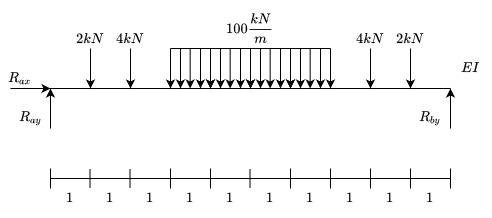
\includegraphics[width=\textwidth]{FBD/FBD_5.jpg}
\caption{Free Body Diagram for Problem 5}
\label{FBD_5}
\end{figure}

With the Free-Body Diagram completed, the report employs the static equations to find the reaction forces at each of the supports as shown in Eq. \ref{problem5_reaction_equation}.

\begin{equation}
\begin{split}
	&\uparrow \sum F_y = R_a - 2 - 4 - 100(4) -4 -2 + R_b = 0 \\
 	&\rightarrow \sum F_x = R_{ax} = 0 \\
 	&\circlearrowleft \sum M_A = -2(1) - 4(2) -100(4)(5) - 4(8) - 2(9) + R_{by}(10) = 0 \\
\end{split}
\label{problem5_reaction_equation}
\end{equation}

Given the problem is statically determinate, the static equations are sufficient to find the reaction forces for the supports, which are shown in Eq. \ref{problem5_reaction_solution}. Since there are no horizontal forces applied, the only non-zero reactionary forces are those in the vertical direction, which will be named $R_a$ and $R_b$ henceforth.

\begin{equation}
\begin{split}
	& R_b = 206 \\
	& R_a = 206 \\
\end{split}
\label{problem5_reaction_solution}
\end{equation}

With the reactions determined, the moment and deflection equations can be constructed as shown in Eq. \ref{problem5_equations}.

\begin{equation}
    \begin{split}
& EI \frac{\delta^2 v}{\delta x^2} = 206\left<x-0\right>^1 - 2\left<x-1\right>^1 -  4\left<x-2\right>^2 - 50\left<x-3\right>^2 + 50\left<x-7\right>^1 \\
& - 2\left<x-8\right>^1 -  4\left<x-9\right>^1 \\
& \\
& EI \frac{\delta v}{\delta x} = 103\left<x-0\right>^2 - \left<x-1\right>^2 -  2\left<x-2\right>^2 - \frac{50}{3}\left<x-3\right>^3 + \frac{50}{3}\left<x-7\right>^3 \\
& - \left<x-8\right>^2 -  2\left<x-9\right>^2  + C_1\\
& \\
& EI v(x) = \frac{103}{3}\left<x-0\right>^3 - \frac{1}{3}\left<x-1\right>^3 -  \frac{2}{3}\left<x-2\right>^3 - \frac{25}{6}\left<x-3\right>^4 + \frac{25}{6}\left<x-7\right>^4 \\
& - \frac{1}{3}\left<x-8\right>^3 -  \frac{2}{3}\left<x-9\right>^3 + C_1x + C_2 \\
    \end{split}
\label{problem5_equations}
\end{equation}

Following the integration of the singularity moment equation, the report solves for the two constants of integration through the use of boundary conditions. As given in the problem description, the two vertical supports at A and B guarantee the deflection at these points is equal to zero, as shown in Eq. \ref{problem5_constants_of_integration}.

\begin{equation}
\begin{split}
	& v(0) = 0 \\
	& v(10) = 0 \\
\end{split}
\label{problem5_constants_of_integration}
\end{equation}

Using the boundary conditions shown above, the report finds the constants of integration to the values shown in Eq. \ref{problem5_constants_of_integration_solution}.

\begin{equation}
\begin{split}
	& C_2 = 0 \\
	& C_1 = \frac{-7223}{3} \\
\end{split}
\label{problem5_constants_of_integration_solution}
\end{equation}

After plugging in the boundary conditions, the report finds the deflection equation shown in Eq. \ref{problem5_final_equation}.

\begin{equation}
\begin{split}
  & EI v(x) = \frac{103}{3}\left<x-0\right>^3 - \frac{1}{3}\left<x-1\right>^3 -  \frac{2}{3}\left<x-2\right>^3 - \frac{25}{6}\left<x-3\right>^4 + \frac{25}{6}\left<x-7\right>^4 \\
& - \frac{1}{3}\left<x-8\right>^3 -  \frac{2}{3}\left<x-9\right>^3 - \frac{-7223}{3}x\\
\end{split}
\label{problem5_final_equation}
\end{equation}



\subsection{Problem 6}

As given by the project assignment, the first project constitutes of a simply supported beam subject to a series of area loads. By substituting the equivalent reaction forces, the report generates the FBD shown in Fig. \ref{prob6:FBD}.

\begin{figure}[h]
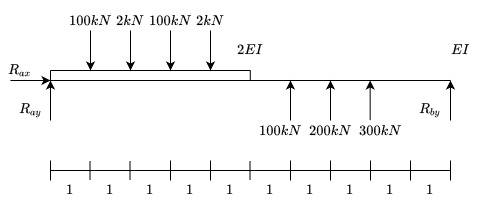
\includegraphics[width=\textwidth]{FBD/FBD_6.jpg}
\caption{Free Body Diagram for Problem 6}
\label{FBD_6}
\end{figure}

With the Free-Body Diagram completed, the report employs the static equations to find the reaction forces at each of the supports as shown in Eq. \ref{problem6_reaction_equation}.

\begin{equation}
\begin{split}
	&\uparrow \sum F_y = R_a - 100 - 2 - 100 -2 + 100 + 200 + 300 + R_b = 0 \\
 	&\rightarrow \sum F_x = R_{ax} = 0 \\
 	&\circlearrowleft \sum M_A = -100(1) - 2(2) -100(3) - 2(4) +100(6) + 200(7) + 300(8) + R_{by}(10) = 0 \\
\end{split}
\label{problem6_reaction_equation}
\end{equation}

Given the problem is statically determinate, the static equations are sufficient to find the reaction forces for the supports, which are shown in Eq. \ref{problem6_reaction_solution}. Since there are no horizontal forces applied, the only non-zero reactionary forces are those in the vertical direction, which will be named $R_a$ and $R_b$ henceforth.

\begin{equation}
\begin{split}
	& R_b = -\frac{1994}{5} \\
	& R_a = \frac{14}{5} \\
\end{split}
\label{problem6_reaction_solution}
\end{equation}

Unlike previous problem, the beam's Modulus of Elasticity $E$ and Area Moment of Inertia $I$ vary throughout the beam. As such, prior to writing the moment and deflection equations, we must first construct an equivalent Free Body Diagram by adding forces and moments. The original shear force and moment diagrams are shown in Fig. \ref{noneq6}.

\begin{figure}[h]
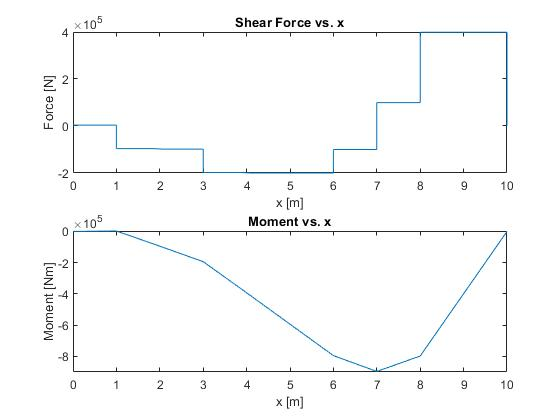
\includegraphics[width=\textwidth]{results/noneq6.jpg}
\caption{Shear Force and Moment Diagrams assuming $EI$ for non-constant $EI$.}
\label{noneq6}
\end{figure}

As given in Fig. \ref{FBD_6}, at the interval $0<x<5$, the beam has the term $2EI$ compared to the interval $5<x<10$ with the term $EI$. To construct the equivalent diagram, the report will multiply all the forces acting on the right side ($x>5$) by two such that the $EI$ terms match, creating Fig. \ref{eq6} with constant $EI$.

\begin{figure}[h]
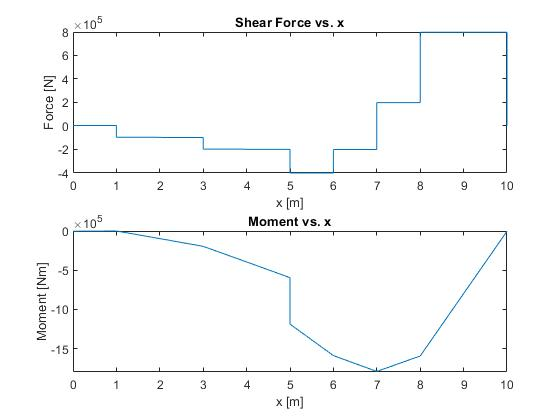
\includegraphics[width=\textwidth]{results/eq6.jpg}
\caption{Shear Force and Moment Diagrams for constant $EI$}
\label{eq6}
\end{figure}

With the equivalent Shear Force and Moment Diagrams, the report constructs a new FBD with an equivalent stiffness $2EI$ shown in Fig. \ref{FBD_6_new}. The FBD will be used to generate the displacement equations shown in Eq. \ref{problem6_equations}.

\begin{figure}[h]
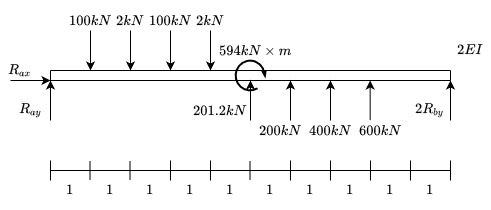
\includegraphics[width=\textwidth]{FBD/FBD_6_new.jpg}
\caption{Free Body Diagram for Problem 6 with Equivalent Stiffness}
\label{FBD_6_new}
\end{figure}

\begin{equation}
    \begin{split}
& 2EI \frac{\delta^2 v}{\delta x^2} = \frac{14}{5}\left<x-0\right>^1 - 100\left<x-1\right>^1 -  2\left<x-2\right>^1 - 100\left<x-3\right>^1 - 2\left<x-4\right>^1 \\
& - \frac{1006}{5}\left<x-5\right>^1 - 594\left<x-5\right>^0 + 200\left<x-6\right>^1 + 400\left<x-7\right>^1 + 600\left<x-8\right>^1 \\
& \\
& 2EI \frac{\delta v}{\delta x} = \frac{7}{5}\left<x-0\right>^2 - 50\left<x-1\right>^2 -  1\left<x-2\right>^2 - 50\left<x-3\right>^2 - \left<x-4\right>^2 \\
& - \frac{503}{5}\left<x-5\right>^2 - 594\left<x-5\right>^1 + 100\left<x-6\right>^2 + 200\left<x-7\right>^2 + 300\left<x-8\right>^2 + C_1 \\
& \\
& 2EI v(x) = \frac{7}{15}\left<x-0\right>^3 - \frac{50}{3}\left<x-1\right>^3 -  \frac{1}{3}\left<x-2\right>^3 - \frac{50}{3}\left<x-3\right>^3 - \frac{1}{3}\left<x-4\right>^3 \\
& - \frac{503}{15}\left<x-5\right>^3 - 297\left<x-5\right>^2 + \frac{100}{3}\left<x-6\right>^3 + \frac{200}{3}\left<x-7\right>^2 + 100\left<x-8\right>^3 + C_1x + C_2\\
    \end{split}
\label{problem6_equations}
\end{equation}

Following the integration of the singularity moment equation, the report solves for the two constants of integration through the use of boundary conditions. As given in the problem description, the two vertical supports at A and B guarantee the deflection at these points is equal to zero, as shown in Eq. \ref{problem6_constants_of_integration}.

\begin{equation}
\begin{split}
	& v(0) = 0 \\
	& v(10) = 0 \\
\end{split}
\label{problem6_constants_of_integration}
\end{equation}

Using the boundary conditions shown above, the report finds the constants of integration to the values shown in Eq. \ref{problem6_constants_of_integration_solution}.

\begin{equation}
\begin{split}
	& C_2 = 0 \\
	& C_1 = \frac{12263}{5} \\
\end{split}
\label{problem6_constants_of_integration_solution}
\end{equation}

After plugging in the boundary conditions, the report finds the deflection equation shown in Eq. \ref{problem6_final_equation}.

\begin{equation}
\begin{split}
  & 2EI v(x) = \frac{7}{15}\left<x-0\right>^3 - \frac{50}{3}\left<x-1\right>^3 -  \frac{1}{3}\left<x-2\right>^3 - \frac{50}{3}\left<x-3\right>^3 - \frac{1}{3}\left<x-4\right>^3 \\
  & - \frac{503}{15}\left<x-5\right>^3 - 297\left<x-5\right>^2 + \frac{100}{3}\left<x-6\right>^3 + \frac{200}{3}\left<x-7\right>^2 + 100\left<x-8\right>^3 + \frac{12263}{5}x\\
\end{split}
\label{problem6_final_equation}
\end{equation}



\subsection{Problem 7}

As given by the project assignment, the first project constitutes of a simply supported beam subject to a series of area loads. By substituting the equivalent reaction forces, the report generates the FBD shown in Fig. \ref{prob7:FBD}.

\begin{figure}[h]
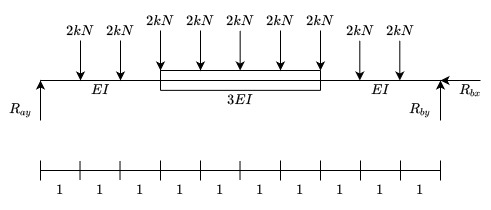
\includegraphics[width=\textwidth]{FBD/FBD_7.jpg}
\caption{Free Body Diagram for Problem 7}
\label{FBD_7}
\end{figure}

With the Free-Body Diagram completed, the report employs the static equations to find the reaction forces at each of the supports as shown in Eq. \ref{problem7_reaction_equation}.

\begin{equation}
\begin{split}
	&\uparrow \sum F_y = R_a - 2 -2 -2 -2 -2 -2 -2 -2 -2 + R_b = 0 \\
 	&\rightarrow \sum F_x = R_{ax} = 0 \\
 	&\circlearrowleft \sum M_A = -2(1) - 2(2) -2(3) - 2(4) -2(5) - 2(6) - 2(7) - 2(8) -2(9) + R_{by}(10) = 0 \\
\end{split}
\label{problem7_reaction_equation}
\end{equation}

Given the problem is statically determinate, the static equations are sufficient to find the reaction forces for the supports, which are shown in Eq. \ref{problem7_reaction_solution}. Since there are no horizontal forces applied, the only non-zero reactionary forces are those in the vertical direction, which will be named $R_a$ and $R_b$ henceforth.

\begin{equation}
\begin{split}
	& R_b = 9 \\
	& R_a = 9 \\
\end{split}
\label{problem7_reaction_solution}
\end{equation}

Unlike previous problem, the beam's Modulus of Elasticity $E$ and Area Moment of Inertia $I$ vary throughout the beam. As such, prior to writing the moment and deflection equations, we must first construct an equivalent Free Body Diagram by adding forces and moments. The original shear force and moment diagrams are shown in Fig. \ref{noneq7}.

\begin{figure}[h]
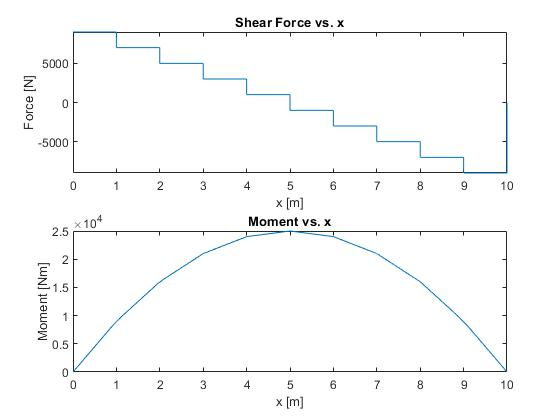
\includegraphics[width=\textwidth]{results/noneq7.jpg}
\caption{Shear Force and Moment Diagrams assuming $EI$ for non-constant $EI$.}
\label{noneq7}
\end{figure}

As given in Fig. \ref{FBD_7}, at the interval $0<x<3$ and $7<x<10$, the beam has the term $EI$ compared to the interval $3<x<7$ with term $3EI$. To construct the equivalent diagram, the report will multiply all the where the term $EI$ is present by three such that the $EI$ terms match, creating Fig. \ref{eq7} with constant $EI$.

\begin{figure}[h]
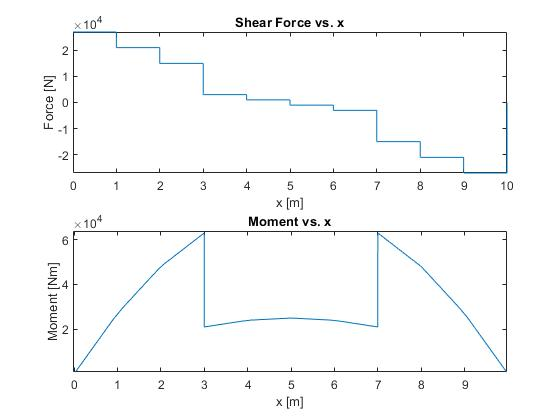
\includegraphics[width=\textwidth]{results/eq7.jpg}
\caption{Shear Force and Moment Diagrams for constant $EI$}
\label{eq7}
\end{figure}

With the equivalent Shear Force and Moment Diagrams, the report constructs a new FBD with an equivalent stiffness $3EI$ shown in Fig. \ref{FBD_7_new}. The FBD will be used to generate the displacement equations shown in Eq. \ref{problem7_equations}.

\begin{figure}[h]
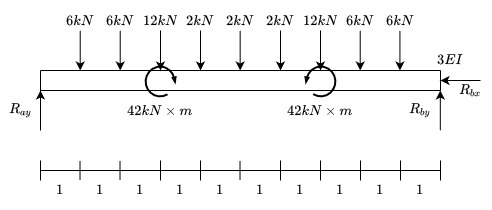
\includegraphics[width=\textwidth]{FBD/FBD_7_new.jpg}
\caption{Free Body Diagram for Problem 7 with Equivalent Stiffness}
\label{FBD_7_new}
\end{figure}

\begin{equation}
    \begin{split}
& 3EI \frac{\delta^2 v}{\delta x^2} = 27\left<x-0\right>^1 - 6\left<x-1\right>^1 - 6\left<x-2\right>^1 - 12\left<x-3\right>^1 - 42\left<x-3\right>^0 - 2\left<x-4\right>^1 \\
& - 2\left<x-5\right>^1 - 2\left<x-6\right>^1 - 12\left<x-7\right>^1 + 42\left<x-7\right>^0 - 6\left<x-8\right>^1 - 6\left<x-9\right>^1 \\
& \\
& 3EI \frac{\delta v}{\delta x} = \frac{27}{2}\left<x-0\right>^2 - 3\left<x-1\right>^2 - 3\left<x-2\right>^2 - 6\left<x-3\right>^2 - 42\left<x-3\right>^1 - \left<x-4\right>^2 \\
& - \left<x-5\right>^2 - \left<x-6\right>^2 - 6\left<x-7\right>^2 + 42\left<x-7\right>^1 - 3\left<x-8\right>^2 - 3\left<x-9\right>^2 + C_1 \\
& \\
& 3EI v(x) = \frac{9}{2}\left<x-0\right>^3 - \left<x-1\right>^3 - \left<x-2\right>^3 - 2\left<x-3\right>^3 - 21\left<x-3\right>^2 - \frac{1}{3}\left<x-4\right>^3 \\
& - \frac{1}{3}\left<x-5\right>^3 - \frac{1}{3}\left<x-6\right>^3 - 2\left<x-7\right>^3 + 21\left<x-7\right>^2 - \left<x-8\right>^3 - \left<x-9\right>^3 + C_1x + C_2 \\
    \end{split}
\label{problem7_equations}
\end{equation}

Following the integration of the singularity moment equation, the report solves for the two constants of integration through the use of boundary conditions. As given in the problem description, the two vertical supports at A and B guarantee the deflection at these points is equal to zero, as shown in Eq. \ref{problem7_constants_of_integration}.

\begin{equation}
\begin{split}
	& v(0) = 0 \\
	& v(10) = 0 \\
\end{split}
\label{problem7_constants_of_integration}
\end{equation}

Using the boundary conditions shown above, the report finds the constants of integration to the values shown in Eq. \ref{problem7_constants_of_integration_solution}.

\begin{equation}
\begin{split}
	& C_2 = 0 \\
	& C_1 = \frac{-307}{2} \\
\end{split}
\label{problem7_constants_of_integration_solution}
\end{equation}

After plugging in the boundary conditions, the report finds the deflection equation shown in Eq. \ref{problem7_final_equation}.

\begin{equation}
\begin{split}
  & 3EI v(x) = \frac{3}{2}\left<x-0\right>^3 - \left<x-1\right>^3 - \left<x-2\right>^3 - 2\left<x-3\right>^3 - 21\left<x-3\right>^2 - \frac{1}{3}\left<x-4\right>^3 \\
& - \frac{1}{3}\left<x-5\right>^3 - \frac{1}{3}\left<x-6\right>^3 - 2\left<x-7\right>^3 + 21\left<x-7\right>^2 - \left<x-8\right>^3 - \left<x-9\right>^3 -   \frac{307}{2}x\\
\end{split}
\label{problem7_final_equation}
\end{equation}

\section{Results}\label{Results}
\subsection{Problem 1}
\begin{figure}[H]
\centering
   \begin{subfigure}[b]{\textwidth}
   \centering
   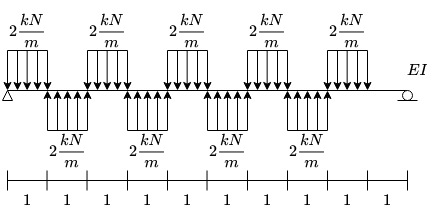
\includegraphics[width=0.7\textwidth]{problems/prob_1.jpg}
   \caption{Given Diagram for Problem 1}
   \label{prob1:prob} 
\end{subfigure}
\begin{subfigure}[b]{\textwidth}
   \centering   
   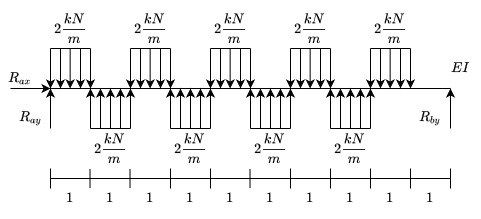
\includegraphics[width=0.8\textwidth]{FBD/FBD_1.jpg}
   \caption{Free Body Diagram for Problem 1}
   \label{prob1:FBD}
\end{subfigure}
\begin{subfigure}[b]{\textwidth}
   \centering   
   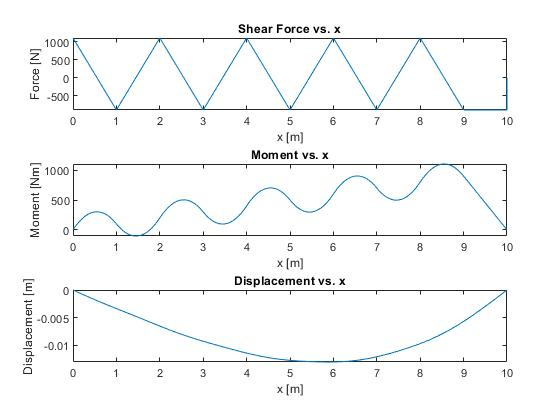
\includegraphics[width=0.87\textwidth]{results/solution_1.jpg}
   \caption{Shear Force, Moment, and Displacement Diagram for Problem 1}
   \label{prob1:results}
\end{subfigure}
\label{prob1}
\end{figure}

Using the deflection equation, the report finds the maximum displacement occurs at $x = 5.8959 m$, which has a downward displacement of $6353.0/EI$ as shown in Fig. \ref{prob1:results}. Given the maximum displacement allowed $v_a = L/500$, or 0.02 meters, and a maximum yield stress of 276 MPa, the report uses Eq. \ref{problem1_beam_geo} and a safety factor $k=1.5$ to find the required Moment of Inertia $I$ of the beam. As such, the W410 X 85 I-Beam would satisfy both the strength and stiffness requirements with a Moment of Inertia $I=17.9 * 10^6\,{mm}^4$.

\begin{equation}
\begin{split}
& I > \frac{v_{max}}{Ev_a} \\
& I > 4.544 * 10^6\,{mm}^2 \\
& I > \frac{M_{max}}{\frac{1}{2}\sigma_{allowed}} = \frac{M_{max}}{\frac{1}{2}\sigma_Y/ k}\\
& I > 11.984 * 10^6\,{mm}^2 \\
\end{split}
\label{problem1_beam_geo}
\end{equation}



\subsection{Problem 2}
\begin{figure}[H]
\centering
   \begin{subfigure}[b]{\textwidth}
   \centering
   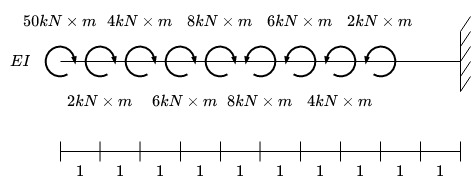
\includegraphics[width=0.7\textwidth]{problems/prob_2.jpg}
   \caption{Given Diagram for Problem 2}
   \label{prob2:prob} 
\end{subfigure}
\begin{subfigure}[b]{\textwidth}
   \centering   
   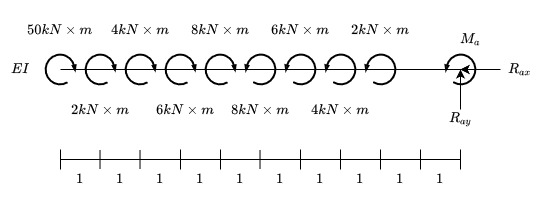
\includegraphics[width=0.8\textwidth]{FBD/FBD_2.jpg}
   \caption{Free Body Diagram for Problem 2}
   \label{prob2:FBD}
\end{subfigure}
\begin{subfigure}[b]{\textwidth}
   \centering   
   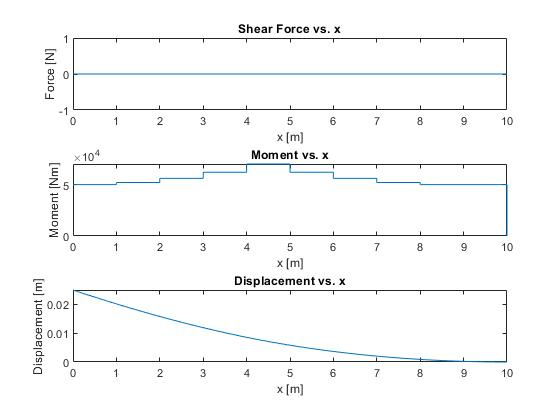
\includegraphics[width=0.87\textwidth]{results/solution_2.jpg}
   \caption{Shear Force, Moment, and Displacement Diagram for Problem 2}
   \label{prob2:results}
\end{subfigure}
\label{prob2}
\end{figure}

Using the deflection equation, the report finds the maximum displacement occurs at $x = 0 m$, which has a downward displacement of $2770000/EI$ as shown in Fig. \ref{prob2:results}. Given the maximum displacement allowed $v_a = L/400$, or 0.025 meters, and a maximum yield stress of 276 MPa, the report uses Eq. \ref{problem2_beam_geo} and a safety factor $k=1.5$ to find the required Moment of Inertia $I$ of the beam. As such, any radius $c$ greater than $0.2120$ meters will suffice.


\begin{equation}
\begin{split}
& \frac{\pi r^4}{4} > \frac{v_{max}}{Ev_a} \\
& r > 0.2120\,m \\
& \frac{\pi r^4}{4} > \frac{M_{max}}{\frac{1}{2}\sigma_Y/ k}\\
& r > 0.1764\,m \\
\end{split}
\label{problem2_beam_geo}
\end{equation}


\subsection{Problem 3}
\begin{figure}[H]
\centering
   \begin{subfigure}[b]{\textwidth}
   \centering
   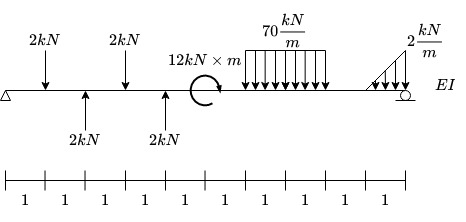
\includegraphics[width=0.7\textwidth]{problems/prob_3.jpg}
   \caption{Given Diagram for Problem 3}
   \label{prob3:prob} 
\end{subfigure}
\begin{subfigure}[b]{\textwidth}
   \centering   
   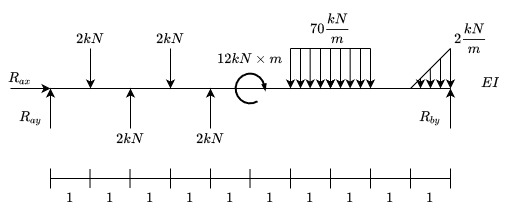
\includegraphics[width=0.8\textwidth]{FBD/FBD_3.jpg}
   \caption{Free Body Diagram for Problem 3}
   \label{prob3:FBD}
\end{subfigure}
\begin{subfigure}[b]{\textwidth}
   \centering   
   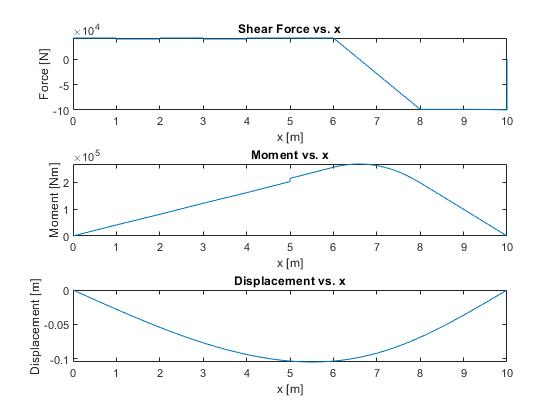
\includegraphics[width=0.87\textwidth]{results/solution_3.jpg}
   \caption{Shear Force, Moment, and Displacement Diagram for Problem 3}
   \label{prob3:results}
\end{subfigure}
\label{prob3}
\end{figure}

Using the deflection equation, the report finds the maximum displacement occurs at $x = 5.5155 m$, which has a downward displacement of $-2289467/EI$ as shown in Fig. \ref{prob3:results}. Assuming the beam chosen is a circular beam with a radius of $c=0.2467$ Moment of Inertia $I=312 * 10^6\,{mm}^4$, the shear force, moment, and displacement can be seen in Fig. \ref{prob3:results}.


\subsection{Problem 4}
\begin{figure}[H]
\centering
   \begin{subfigure}[b]{\textwidth}
   \centering
   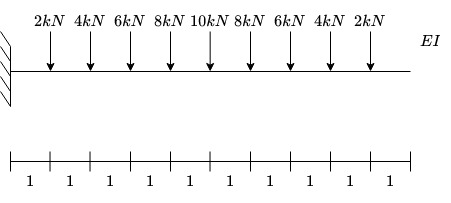
\includegraphics[width=0.7\textwidth]{problems/prob_4.jpg}
   \caption{Given Diagram for Problem 4}
   \label{prob4:prob} 
\end{subfigure}
\begin{subfigure}[b]{\textwidth}
   \centering   
   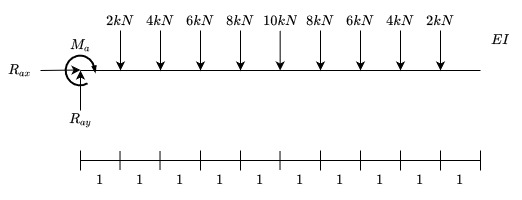
\includegraphics[width=0.8\textwidth]{FBD/FBD_4.jpg}
   \caption{Free Body Diagram for Problem 4}
   \label{prob4:FBD}
\end{subfigure}
\begin{subfigure}[b]{\textwidth}
   \centering   
   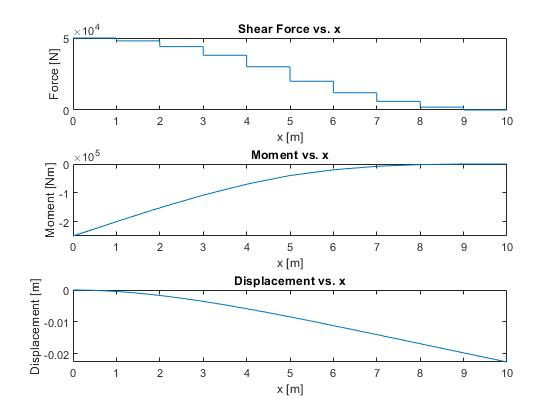
\includegraphics[width=0.87\textwidth]{results/solution_4.jpg}
   \caption{Shear Force, Moment, and Displacement Diagram for Problem 4}
   \label{prob4:results}
\end{subfigure}
\label{prob4}
\end{figure}

Using the deflection equation, the report finds the maximum displacement occurs at $x = 10 m$, which has a downward displacement of $-5708330/EI$ as shown in Fig. \ref{prob2:results}. Given the maximum displacement allowed $v_a = L/400$, or 0.025 meters, and a maximum yield stress of 276 MPa, the report uses Eq. \ref{problem2_beam_geo} and a safety factor $k=1.5$ to find the required Moment of Inertia $I$ of the beam. As such, a circular beam with a radius $c$ greater than $0.2540$ meters will suffice, or a Moment of Inertia $I > 3266.57 * 10^6\,{mm}^4$.


\begin{equation}
\begin{split}
& \frac{\pi r^4}{4} > \frac{v_{max}}{Ev_a} \\
& r > 0.2540\,m \\
& \frac{\pi r^4}{4} > \frac{M_{max}}{\frac{1}{2}\sigma_Y/ k}\\
& r > 0.2606\,m \\
\end{split}
\label{problem4_beam_geo}
\end{equation}



\subsection{Problem 5}
\begin{figure}[H]
\centering
   \begin{subfigure}[b]{\textwidth}
   \centering
   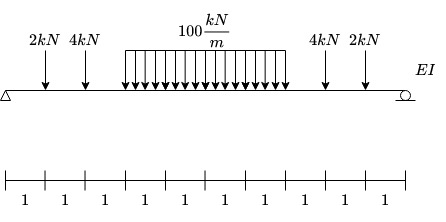
\includegraphics[width=0.7\textwidth]{problems/prob_5.jpg}
   \caption{Given Diagram for Problem 5}
   \label{prob5:prob} 
\end{subfigure}
\begin{subfigure}[b]{\textwidth}
   \centering   
   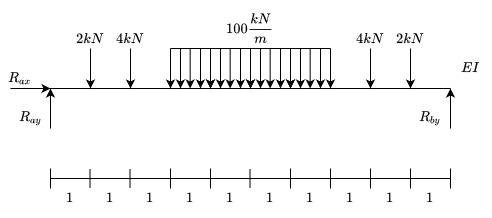
\includegraphics[width=0.8\textwidth]{FBD/FBD_5.jpg}
   \caption{Free Body Diagram for Problem 5}
   \label{prob5:FBD}
\end{subfigure}
\begin{subfigure}[b]{\textwidth}
   \centering   
   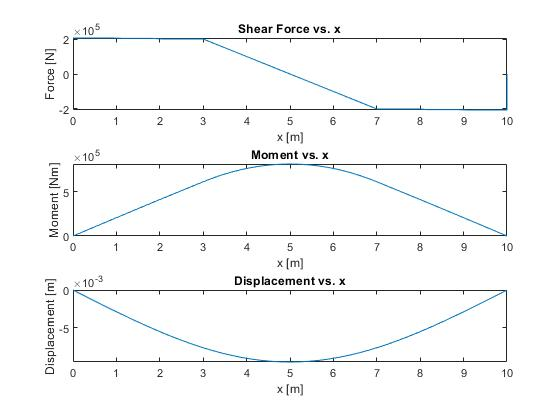
\includegraphics[width=0.87\textwidth]{results/solution_5.jpg}
   \caption{Shear Force, Moment, and Displacement Diagram for Problem 5}
   \label{prob5:results}
\end{subfigure}
\label{prob5}
\end{figure}

Using the deflection equation, the report finds the maximum displacement occurs at $x = 5.0 m$, which has a downward displacement of $-7852656/EI$ as shown in Fig. \ref{prob5:results}. Given the maximum displacement allowed $v_a = L/400$, or 0.025 meters, and a maximum yield stress of 276 MPa as that of an aluminum beam , the report uses Eq. \ref{problem5_beam_geo} and a safety factor $k=1.5$ to find the required Moment of Inertia $I$ of the beam. As such, a circular beam with a radius $c$ greater than $0.3497$ meters will suffice, or a Moment of Inertia $I > 11739.11 * 10^6\,{mm}^4$.

\begin{equation}
\begin{split}
& \frac{\pi r^4}{4} > \frac{v_{max}}{Ev_a} \\
& r > 0.2472\,m \\
& \frac{\pi r^4}{4} > \frac{M_{max}}{\frac{1}{2}\sigma_Y/ k}\\
& r > 0.3497\,m \\
\end{split}
\label{problem5_beam_geo}
\end{equation}

Assuming the beam chosen has a Moment of Inertia $I = 4493.65 * 10^6\,{mm}^4$, the shear force, moment, and displacement can be seen in Fig. \ref{prob5:results} where the maximum displacement occurs exactly at the center of the beam due to symmetry about its midpoint.


\subsection{Problem 6}
\begin{figure}[H]
\centering
   \begin{subfigure}[b]{\textwidth}
   \centering
   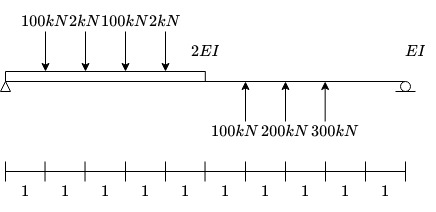
\includegraphics[width=0.7\textwidth]{problems/prob_6.jpg}
   \caption{Given Diagram for Problem 6}
   \label{prob6:prob} 
\end{subfigure}
\begin{subfigure}[b]{\textwidth}
   \centering   
   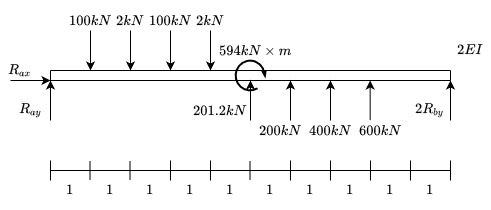
\includegraphics[width=0.8\textwidth]{FBD/FBD_6_new.jpg}
   \caption{Free Body Diagram for Problem 6}
   \label{prob6:FBD}
\end{subfigure}
\begin{subfigure}[b]{\textwidth}
   \centering   
   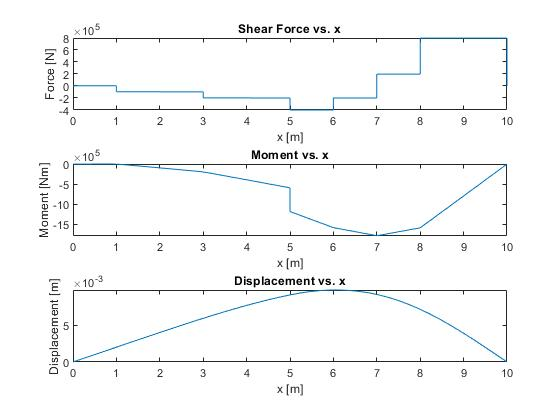
\includegraphics[width=0.87\textwidth]{results/solution_6.jpg}
   \caption{Shear Force, Moment, and Displacement Diagram for Problem 6}
   \label{prob6:results}
\end{subfigure}
\label{prob6}
\end{figure}

Using the deflection equation, the report finds the maximum displacement occurs at $x = 5.0 m$, which has a downward displacement of $11930984/EI$ as shown in Fig. \ref{prob6:results}. Assuming an aluminum beam with a maximum yield stress of 276 MPa, the report uses Eq. \ref{problem6_beam_geo} and a safety factor $k=1.5$ to find the required Moment of Inertia $I$ of the beam. As such, a circular beam with a radius $c$ greater than $0.3969$ meters will suffice, or a Moment of Inertia $I > 19480.35 * 10^6\,{mm}^4$.

\begin{equation}
\begin{split}
& \frac{\pi r^4}{4} > \frac{v_{max}}{Ev_a} \\
& r > 0.3053\,m \\
& \frac{\pi r^4}{4} > \frac{M_{max}}{\frac{1}{2}\sigma_Y/ k}\\
& r > 0.3969\,m \\
\end{split}
\label{problem6_beam_geo}
\end{equation}


\subsection{Problem 7}
\begin{figure}[H]
\centering
   \begin{subfigure}[b]{\textwidth}
   \centering
   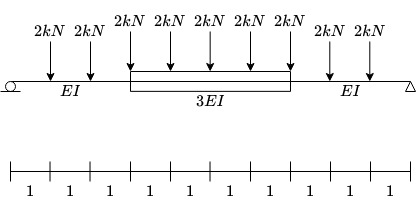
\includegraphics[width=0.7\textwidth]{problems/prob_7.jpg}
   \caption{Given Diagram for Problem 7}
   \label{prob7:prob} 
\end{subfigure}
\begin{subfigure}[b]{\textwidth}
   \centering   
   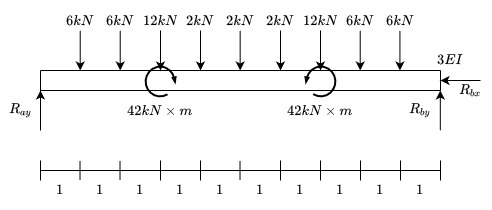
\includegraphics[width=0.8\textwidth]{FBD/FBD_7_new.jpg}
   \caption{Free Body Diagram for Problem 7}
   \label{prob7:FBD}
\end{subfigure}
\begin{subfigure}[b]{\textwidth}
   \centering   
   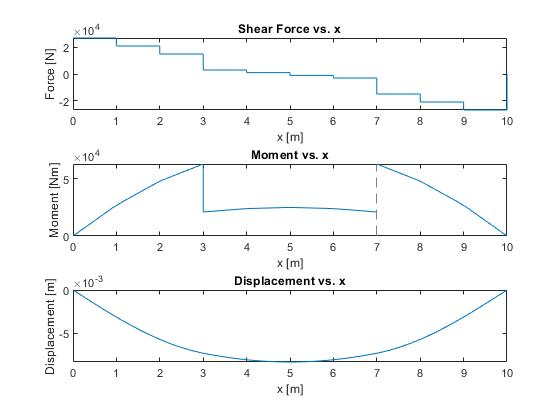
\includegraphics[width=0.87\textwidth]{results/solution_7.jpg}
   \caption{Shear Force, Moment, and Displacement Diagram for Problem 7}
   \label{prob7:results}
\end{subfigure}
\label{prob7}
\end{figure}

Using the deflection equation, the report finds the maximum displacement occurs at $x = 5.0 m$, which has a downward displacement of $396333/EI$ as shown in Fig. \ref{prob7:results}. Assuming an aluminum beam with a maximum yield stress of 276 MPa, the report uses Eq. \ref{problem7_beam_geo} and a safety factor $k=1.5$ to find the required Moment of Inertia $I$ of the beam. As such, a circular beam with a radius $c$ greater than $0.1718$ meters will suffice, or a Moment of Inertia $I > 683.64 * 10^6\,{mm}^4$.

\begin{equation}
\begin{split}
& \frac{\pi r^4}{4} > \frac{v_{max}}{Ev_a} \\
& r > 0.1304\,m \\
& \frac{\pi r^4}{4} > \frac{M_{max}}{\frac{1}{2}\sigma_Y/ k}\\
& r > 0.1718\,m \\
\end{split}
\label{problem7_beam_geo}
\end{equation}

\section{Conclusions} \label{Conclusions}
The project provided excellent practice for real-life working conditions in beam deflection. It is often the case in large projects that communication stands as the greatest barrier towards completion, which was perfectly demonstrated through the project. From discussions of misunderstandings with the professor to design choices based on abstract loads, the project greatly improved my understanding of beam deflection and how to troubleshoot all issues that may arise from it. In addition to the theoretical modeling, the modeling of the beam on MATLAB allowed for the improvement of the ability to convey ideas clearly and objectively.

Future projects should consider decreasing the workload on students by substituting a large number of problems with a complex central problem that incorporates all the required skills; in addition to removing some of the repetition, the problem would more closely model real life's working conditions.
\section{Appendix}
\subsection{Main MATLAB Plotting}
\begin{verbatim*}
%% Header
% Name: Pedro Almeida
% Date: October 1st, 2021
% Course: EGM 4523C – Intermediate Strength of Materials
% Serial Number: 2

%% Preparation
clc; clear; close all;
s = 2;
range_x = [0 10];
run_problems = [72];


%% Problem 1
if any(run_problems(:) == 1)
    figure(1)

    %Constants
    L = 10; %Beam Length
    E = 69.9e9; %Young's Modulus
    v_allowed = L/500; %Allowed Displacement
    k = 1.5; %Safety Factor
    sY = 276e6; %Yield Stress
%     I = 6.95e-6;
    I = 1/E;

    %Problem Solution
    syms x

    %Shear Force Plot
    subplot(3,1,1)
    shear = 1000*(.55*s*pw(x,0,0) -s*pw(x,0,1) + 2*s*pw(x,1,1) - 2*s*pw(x,2,1) + 2*s*pw(x,3,1) - 2*s*pw(x,4,1) + 2*s*pw(x,5,1) - 2*s*pw(x,6,1) + 2*s*pw(x,7,1) - 2*s*pw(x,8,1) + s*pw(x,9,1) + 0.45*s*pw(x,10,0));
    fplot(shear, range_x);
    title('Shear Force vs. x');
    xlabel('x [m]')
    ylabel('Force [N]')

    %Moment Plot
    subplot(3,1,2)
    moment = 1000*(0.55*s*pw(x,0,1) -(s/2)*pw(x,0,2) + 2*(s/2)*pw(x,1,2) - 2*(s/2)*pw(x,2,2) + 2*(s/2)*pw(x,3,2) - 2*(s/2)*pw(x,4,2) + 2*(s/2)*pw(x,5,2) - 2*(s/2)*pw(x,6,2) + 2*(s/2)*pw(x,7,2) - 2*(s/2)*pw(x,8,2) + (s/2)*pw(x,9,2) + 0.45*s*pw(x,10,1));
    fplot(moment, range_x);
    title('Moment vs. x');
    xlabel('x [m]')
    ylabel('Moment [Nm]')

    %Displacement Plot
    subplot(3,1,3)
    displacement = 1000*(0.55*(s/6)*pw(x,0,3) -(s/24)*pw(x,0,4) + 2*(s/24)*pw(x,1,4) - 2*(s/24)*pw(x,2,4) + 2*(s/24)*pw(x,3,4) - 2*(s/24)*pw(x,4,4) + 2*(s/24)*pw(x,5,4) - 2*(s/24)*pw(x,6,4) + 2*(s/24)*pw(x,7,4) - 2*(s/24)*pw(x,8,4) + (s/24)*pw(x,9,4) - (209/240)*s*pw(x,0,1) + 0.45*(s/6)*pw(x,10,3))/(E*I);
    fplot(displacement, range_x);
    title('Displacement vs. x');
    xlabel('x [m]')
    ylabel('Displacement [m]')


    [I1, I2] = getMoment(displacement, range_x, moment, v_allowed, E, sY, k);
    fprintf('Min Area = %f\n',I1);
    fprintf('Min I = %f\n',I2);
end



%% Problem 2
if any(run_problems(:) == 2)
    figure(2)

    %Constants
    L = 10; %Beam Length
    E = 69.9e9; %Young's Modulus
    v_allowed = L/400; %Allowed Displacement
    k = 1.5; %Safety Factor
    sY = 276e6; %Yield Stress
    I=1/E;
%     I = 1585.121602e-6; %

    %Problem Solution
    syms x

    %Shear Force Plot
    subplot(3,1,1)
    shear = 0;
    fplot(shear, range_x);
    title('Shear Force vs. x');
    xlabel('x [m]')
    ylabel('Force [N]')

    %Moment Plot
    subplot(3,1,2)
    moment = 1000*(50*pw(x,0,0) + s*pw(x,1,0) + 2*s*pw(x,2,0) + 3*s*pw(x,3,0) + 4*s*pw(x,4,0) - 4*s*pw(x,5,0) - 3*s*pw(x,6,0) - 2*s*pw(x,7,0) - s*pw(x,8,0) - 50*pw(x,10,0));
    fplot(moment, range_x);
    title('Moment vs. x');
    xlabel('x [m]')
    ylabel('Moment [Nm]')

    %Displacement Plot
    subplot(3,1,3)
    displacement = (1000*(25*pw(x,0,2) + (s/2)*pw(x,1,2) + 2*(s/2)*pw(x,2,2) + 3*(s/2)*pw(x,3,2) + 4*(s/2)*pw(x,4,2) - 4*(s/2)*pw(x,5,2) - 3*(s/2)*pw(x,6,2) - 2*(s/2)*pw(x,7,2) - (s/2)*pw(x,8,2) + (-500 - 30*s)*pw(x,0,1) + (2500 + 135*s) - 25*pw(x,10,2)))/(E*I);
    fplot(displacement, range_x);
    title('Displacement vs. x');
    xlabel('x [m]')
    ylabel('Displacement [m]')

    [I1, I2] = getMoment(displacement, range_x, moment, v_allowed, E, sY, k);
    fprintf('Min Area = %f\n',I1);
    fprintf('Min I = %f\n',I2);
    
    %Min Radius = 0.2120 meters
end

%% Problem 3
if any(run_problems(:) == 3)
    figure(3)

    %Constants
    L = 10; %Beam Length
    E = 69.9e9; %Young's Modulus
    v_allowed = L/400; %Allowed Displacement
    k = 1.5; %Safety Factor
    sY = 276e6; %Yield Stress
    I = 1/E;
    I = 2908.086809e-6; %

    %Problem Solution
    syms x

    %Shear Force Plot
    subplot(3,1,1)
    shear = 1000*(((7*s)/60 + 41)*pw(x,0,0) - s*pw(x,1,0) + s*pw(x,2,0) - s*pw(x,3,0) + s*pw(x,4,0) - 70*pw(x,6,1) + 70*pw(x,8,1) - (s/2)*pw(x,9,2)  + ((23*s)/60 + 99)*pw(x,10,0));
    fplot(shear, range_x);
    title('Shear Force vs. x');
    xlabel('x [m]')
    ylabel('Force [N]')

    %Moment Plot
    subplot(3,1,2)
    moment = 1000*(((7*s)/60 + 41)*pw(x,0,1) - s*pw(x,1,1) + s*pw(x,2,1) - s*pw(x,3,1) + s*pw(x,4,1) + (s+10)*pw(x,5,0) - 35*pw(x,6,2) + 35*pw(x,8,2) - (s/6)*pw(x,9,3) + ((23*s)/60 + 99)*pw(x,10,1));
    fplot(moment, range_x);
    title('Moment vs. x');
    xlabel('x [m]')
    ylabel('Moment [Nm]')

    %Displacement Plot
    subplot(3,1,3)
    displacement = (1000*((((7*s)/60 + 41)/6)*pw(x,0,3) - (s/6)*pw(x,1,3) + (s/6)*pw(x,2,3) - (s/6)*pw(x,3,3) + (s/6)*pw(x,4,3) + ((s+10)/2)*pw(x,5,2) - (35/12)*pw(x,6,4) + (35/12)*pw(x,8,4) - (s/120)*pw(x,9,5) + ((9143*s)/3600 - (3755/6))*pw(x,0,1) + (((23*s)/60 + 99)/6)*pw(x,10,3)))/(E*I);
    fplot(displacement, range_x);
    title('Displacement vs. x');
    xlabel('x [m]')
    ylabel('Displacement [m]')

    [A, I] = getMoment(displacement, range_x, moment, v_allowed, E, sY, k);
    fprintf('Min Area = %f\n',A);
    fprintf('Min I = %f\n',I);
end


%% Problem 4
if any(run_problems(:) == 4)
    figure(4)

    %Constants
    L = 10; %Beam Length
    E = 69.9e9; %Young's Modulus
    v_allowed = L/400; %Allowed Displacement
    k = 2; %Safety Factor
    sY = 276e6; %Yield Stress
    I = 1/E;
    I = 3623.188406e-6; %

    %Problem Solution
    syms x

    %Shear Force Plot
    subplot(3,1,1)
    shear = 1000*(25*s*pw(x,0,0) - s*pw(x,1,0) - 2*s*pw(x,2,0) - 3*s*pw(x,3,0) - 4*s*pw(x,4,0) - 5*s*pw(x,5,0) - 4*s*pw(x,6,0) - 3*s*pw(x,7,0) - 2*s*pw(x,8,0) - s*pw(x,9,0));
    fplot(shear, range_x);
    title('Shear Force vs. x');
    xlabel('x [m]')
    ylabel('Force [N]')

    %Moment Plot
    subplot(3,1,2)
    moment = 1000*(25*s*pw(x,0,1) - 125*s*pw(x,0,0) - s*pw(x,1,1) - 2*s*pw(x,2,1) - 3*s*pw(x,3,1) - 4*s*pw(x,4,1) - 5*s*pw(x,5,1) - 4*s*pw(x,6,1) - 3*s*pw(x,7,1) - 2*s*pw(x,8,1) - s*pw(x,9,1));
    fplot(moment, range_x);
    title('Moment vs. x');
    xlabel('x [m]')
    ylabel('Moment [Nm]')

    %Displacement Plot
    subplot(3,1,3)
    displacement = (1000*((25/6)*s*pw(x,0,3) - (125/2)*s*pw(x,0,2) - (s/6)*pw(x,1,3) - 2*(s/6)*pw(x,2,3) - 3*(s/6)*pw(x,3,3) - 4*(s/6)*pw(x,4,3) - 5*(s/6)*pw(x,5,3) - 4*(s/6)*pw(x,6,3) - 3*(s/6)*pw(x,7,3) - 2*(s/6)*pw(x,8,3) - (s/6)*pw(x,9,3)))/(E*I);
    fplot(displacement, range_x);
    title('Displacement vs. x');
    xlabel('x [m]')
    ylabel('Displacement [m]')

    [A, I] = getMoment(displacement, range_x, moment, v_allowed, E, sY, k);
    fprintf('Min Area = %f\n',A);
    fprintf('Min I = %f\n',I);
end


%% Problem 5
if any(run_problems(:) == 5)
    figure(5)

    %Constants
    L = 10; %Beam Length
    E = 69.9e9; %Young's Modulus
    v_allowed = L/400; %Allowed Displacement
    k = 2; %Safety Factor
    sY = 276e6; %Yield Stress
    I = 1/E; %
    I = 11739.112283e-6;

    %Problem Solution
    syms x

    %Shear Force Plot
    subplot(3,1,1)
    shear = 1000*((3*s + 200)*pw(x,0,0) - s*pw(x,1,0) - 2*s*pw(x,2,0) - 100*pw(x,3,1) + 100*pw(x,7,1) - 2*s*pw(x,8,0)- s*pw(x,9,0) + (3*s+200)*pw(x,10,0));
    fplot(shear, range_x);
    title('Shear Force vs. x');
    xlabel('x [m]')
    ylabel('Force [N]')

    %Moment Plot
    subplot(3,1,2)
    moment = 1000*((3*s + 200)*pw(x,0,1) - s*pw(x,1,1) - 2*s*pw(x,2,1) - 50*pw(x,3,2) + 50*pw(x,7,2) - 2*s*pw(x,8,1)- s*pw(x,9,1) + (3*s+200)*pw(x,10,1));
    fplot(moment, range_x);
    title('Moment vs. x');
    xlabel('x [m]')
    ylabel('Moment [Nm]')

    %Displacement Plot
    subplot(3,1,3)
    displacement = (1000*(((3*s + 200)/6)*pw(x,0,3) - (s/6)*pw(x,1,3) - 2*(s/6)*pw(x,2,3) - (25/6)*pw(x,3,4) + (25/6)*pw(x,7,4) - 2*(s/6)*pw(x,8,3)- (s/6)*pw(x,9,3) + (-(41*s)/2 - 7100/3)*pw(x,0,1) + ((3*s+200)/6)*pw(x,10,3)))/(E*I);
    fplot(displacement, range_x);
    title('Displacement vs. x');
    xlabel('x [m]')
    ylabel('Displacement [m]')

    [A, I] = getMoment(displacement, range_x, moment, v_allowed, E, sY, k);
    fprintf('Min Area = %f\n',A);
    fprintf('Min I = %f\n',I);
end


%% Problem 6_1
if any(run_problems(:) == 61)
    figure(6)

    %Constants
    L = 10; %Beam Length
    E = 69.9e9; %Young's Modulus
    v_allowed = L/400; %Allowed Displacement
    k = 1.5; %Safety Factor
    sY = 276e6; %Yield Stress
    I = 0; %

    %Problem Solution
    syms x

    %Shear Force Plot
    subplot(2,1,1)
    shear = 1000*(((7*s)/5)*pw(x,0,0) - 100*pw(x,1,0) - s*pw(x,2,0) - 100*pw(x,3,0) - s*pw(x,4,0) + 100*pw(x,6,0) + 200*pw(x,7,0) + 300*pw(x,8,0) + (((3*s)/5) - 400)*pw(x,10,0));
    fplot(shear, range_x);
    title('Shear Force vs. x');
    xlabel('x [m]')
    ylabel('Force [N]')

    %Moment Plot
    subplot(2,1,2)
    moment = 1000*(((7*s)/5)*pw(x,0,1) - 100*pw(x,1,1) - s*pw(x,2,1) - 100*pw(x,3,1) - s*pw(x,4,1) + 100*pw(x,6,1) + 200*pw(x,7,1) + 300*pw(x,8,1) + (((3*s)/5) - 400)*pw(x,10,1));
    fplot(moment, range_x);
    title('Moment vs. x');
    xlabel('x [m]')
    ylabel('Moment [Nm]')
end

%% Problem 6_2
if any(run_problems(:) == 62)
    figure(7)

    %Constants
    L = 10; %Beam Length
    E = 69.9e9; %Young's Modulus
    v_allowed = L/400; %Allowed Displacement
    k = 1.5; %Safety Factor
    sY = 276e6; %Yield Stress
%     I = 1/E;
    I = 19480.349915e-6;

    %Problem Solution
    syms x

    %Shear Force Plot
    subplot(3,1,1)
    shear = 1000*(((7*s)/5)*pw(x,0,0) - 100*pw(x,1,0) - s*pw(x,2,0) - 100*pw(x,3,0) - s*pw(x,4,0) - ((3*s)/5 + 200)*pw(x,5,0) + 2*100*pw(x,6,0) + 2*200*pw(x,7,0) + 2*300*pw(x,8,0) + 2*(((3*s)/5) - 400)*pw(x,10,0));
    fplot(shear, range_x);
    title('Shear Force vs. x');
    xlabel('x [m]')
    ylabel('Force [N]')

    %Moment Plot
    subplot(3,1,2)
    moment = 1000*(((7*s)/5)*pw(x,0,1) - 100*pw(x,1,1) - s*pw(x,2,1) - 100*pw(x,3,1) - s*pw(x,4,1) - ((3*s)/5 + 200)*pw(x,5,1) + (3*s - 600)*pw(x,5,0) + 2*100*pw(x,6,1) + 2*200*pw(x,7,1) + 2*300*pw(x,8,1) + 2*(((3*s)/5) - 400)*pw(x,10,1));
    fplot(moment, range_x);
    title('Moment vs. x');
    xlabel('x [m]')
    ylabel('Moment [Nm]')
    
    %Displacement Plot
    subplot(3,1,3)
    displacement = (1000*(((7*s)/30)*pw(x,0,3) - (100/6)*pw(x,1,3) - (s/6)*pw(x,2,3) - (100/6)*pw(x,3,3) - (s/6)*pw(x,4,3) - (((3*s)/5 + 200)/6)*pw(x,5,3) + ((3*s - 600)/2)*pw(x,5,2) + 2*(100/6)*pw(x,6,3) + 2*(200/6)*pw(x,7,3) + 2*(300/6)*pw(x,8,3) + (-(137*s)/10 + 2480)*pw(x,0,1) + 2*((((3*s)/5) - 400)/6)*pw(x,10,3)))/(10*E*I);
    fplot(displacement, range_x);
    title('Displacement vs. x');
    xlabel('x [m]')
    ylabel('Displacement [m]')

    [A, I] = getMoment(displacement, range_x, moment, v_allowed, E, sY, k);
    fprintf('Min Area = %f\n',A);
    fprintf('Min I = %f\n',I);
end


%% Problem 7_1
if any(run_problems(:) == 71)
    figure(8)

    %Constants
    L = 10; %Beam Length
    E = 69.9e9; %Young's Modulus
    v_allowed = L/400; %Allowed Displacement
    k = 1.5; %Safety Factor
    sY = 276e6; %Yield Stress
    I = 0; %

    %Problem Solution
    syms x

    %Shear Force Plot
    subplot(2,1,1)
    shear = 1000*(4.5*s*pw(x,0,0) - s*pw(x,1,0) - s*pw(x,2,0) - s*pw(x,3,0) - s*pw(x,4,0) - s*pw(x,5,0) - s*pw(x,6,0) - s*pw(x,7,0) - s*pw(x,8,0) - s*pw(x,9,0) + 4.5*s*pw(x,10,0));
    fplot(shear, range_x);
    title('Shear Force vs. x');
    xlabel('x [m]')
    ylabel('Force [N]')

    %Moment Plot
    subplot(2,1,2)
    moment = 1000*(4.5*s*pw(x,0,1) - s*pw(x,1,1) - s*pw(x,2,1) - s*pw(x,3,1) - s*pw(x,4,1) - s*pw(x,5,1) - s*pw(x,6,1) - s*pw(x,7,1) - s*pw(x,8,1) - s*pw(x,9,1) + 4.5*s*pw(x,10,1));
    fplot(moment, range_x);
    title('Moment vs. x');
    xlabel('x [m]')
    ylabel('Moment [Nm]')
end

%% Problem 7_2
if any(run_problems(:) == 72)
    figure(9)

    %Constants
    L = 10; %Beam Length
    E = 69.9e9; %Young's Modulus
    v_allowed = L/400; %Allowed Displacement
    k = 1.5; %Safety Factor
    sY = 276e6; %Yield Stress
%     I = 1/(3*E);
    I = 683.640162e-6/3;

    %Problem Solution
    syms x

    %Shear Force Plot
    subplot(3,1,1)
    shear = 1000*(3*4.5*s*pw(x,0,0) - 3*s*pw(x,1,0) - 3*s*pw(x,2,0) - s*pw(x,3,0) - 5*s*pw(x,3,0) - s*pw(x,4,0) - s*pw(x,5,0) - s*pw(x,6,0) - s*pw(x,7,0) - 5*s*pw(x,7,0) - 3*s*pw(x,8,0) - 3*s*pw(x,9,0) + 3*4.5*s*pw(x,10,0));
    fplot(shear, range_x);
    title('Shear Force vs. x');
    xlabel('x [m]')
    ylabel('Force [N]')

    %Moment Plot
    subplot(3,1,2)
    moment = 1000*(3*4.5*s*pw(x,0,1) - 3*s*pw(x,1,1) - 3*s*pw(x,2,1) - s*pw(x,3,1) - 5*s*pw(x,3,1) - 21*s*pw(x,3,0) - s*pw(x,4,1) - s*pw(x,5,1) - s*pw(x,6,1) - s*pw(x,7,1) - 5*s*pw(x,7,1) + 21*s*pw(x,7,0) - 3*s*pw(x,8,1) - 3*s*pw(x,9,1) + 3*4.5*s*pw(x,10,1));
    fplot(moment, range_x);
    title('Moment vs. x');
    xlabel('x [m]')
    ylabel('Moment [Nm]')
    
    %Displacement Plot
    subplot(3,1,3)
    displacement = (1000*(3*4.5*(1/6)*s*pw(x,0,3) - 3*(1/6)*s*pw(x,1,3) - 3*(1/6)*s*pw(x,2,3) - s*(1/6)*pw(x,3,3) - 5*(1/6)*s*pw(x,3,3) - 21*(1/2)*s*pw(x,3,2) - s*(1/6)*pw(x,4,3) - s*(1/6)*pw(x,5,3) - s*(1/6)*pw(x,6,3) - s*(1/6)*pw(x,7,3) - 5*(1/6)*s*pw(x,7,3) + 21*(1/2)*s*pw(x,7,2) - 3*(1/6)*s*pw(x,8,3) - 3*(1/6)*s*pw(x,9,3) + (-76.75 * s)*pw(x,0,1) + 3*4.5*(1/6)*s*pw(x,10,3)))/(3*E*I);
    fplot(displacement, range_x);
    title('Displacement vs. x');
    xlabel('x [m]')
    ylabel('Displacement [m]')

    [A, I] = getMoment(displacement, range_x, moment, v_allowed, E, sY, k);
    fprintf('Min Area = %f\n',A);
    fprintf('Min I = %f\n',I);
end
\end{verbatim*}
\subsection{Piecewise Function}
\begin{verbatim*}
function out = pw(x,x0,n)
    out = piecewise(x>=x0, (x-x0)^n, 0);
end
\end{verbatim*}


\subsection{getMoment Function}
\begin{verbatim*}
function [I1, I2] = getMoment(displacement, range_x, moment, v_allowed, E, sY, k)
    
    Sa = sY / k;

    [~, a, ~, b] = getMax(moment, range_x);
    M = max(abs(a), abs(b));
    
    I1 = M/((1/2) * Sa) * 10^6;

    disp(M)

    [~, c, ~, d] = getMax(displacement, range_x);
    v = max(abs(c), abs(d));

    disp(v)

    I2 = v/(E*v_allowed) * 10^6;
end
\end{verbatim*}
\subsection{getRadius Function}
\begin{verbatim*}
function r = getRadius(I)
    r = ((I * 10^-6 * 4)/pi)^(1/4);
end
\end{verbatim*}


\subsection{getMax Function}
\begin{verbatim*}
function [x1, mins, x2, maxs] = getMax(f, range)
    domain = linspace(range(1), range(2), 1000);

    disps = subs(f, domain);

    [mins, i1] = min(disps);
    [maxs, i2] = max(disps);

    x1 = domain(i1);
    x2 = domain(i2);

end
\end{verbatim*}

\bibliographystyle{ieeetr}
\bibliography{ref}

\end{document}
